\section{AutoLibra\protect\includegraphics[height=1em]{figs/scale.png}}

\begin{figure}[!t]
    \centering
    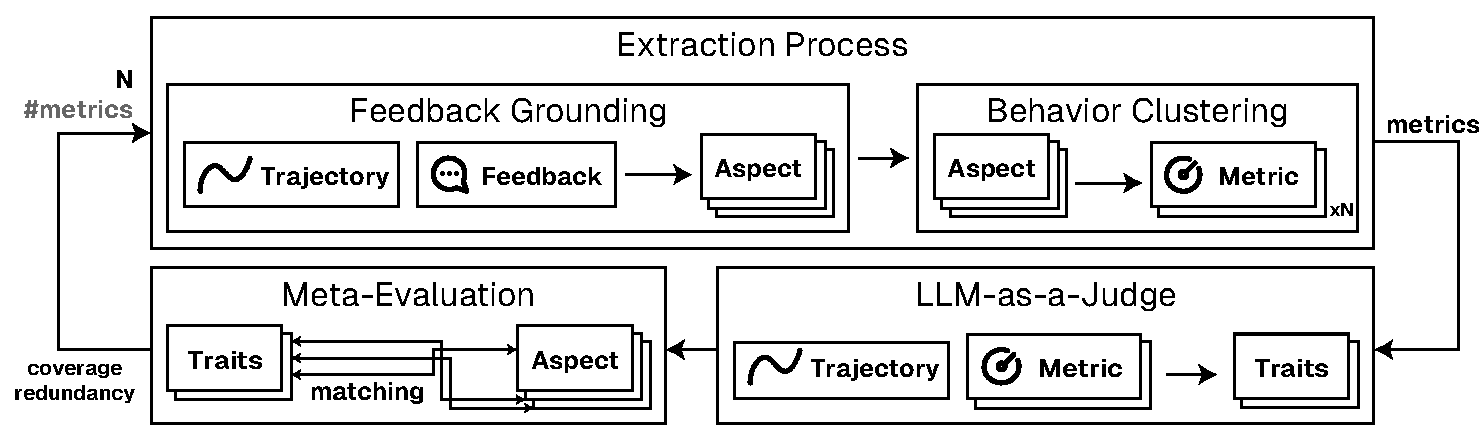
\includegraphics[width=\textwidth]{figs/autolibra-pipeline.pdf}
    \caption{AutoLibra pipeline. AutoLibra consists of three major components: Extraction Process
    turns annotated agent trajectories into metrics, LLM-as-a-Judge evaluates the agent trajectories
    based on the induced metrics, and Meta-Evaluation Process measures the quality of induced metrics
    through matching the detect agent traits with grounded feedback aspects.
    }
    \label{fig:autolibra-pipeline}
\end{figure}

To address the limitations of existing evaluation paradigms, we seek to design an evaluation method that 
meets the following desiderata: (1) \emph{data-driven}: this makes sure that the metrics are grounded
in the real agent behavior and human opinions, (2) \emph{generic}: applicable to various agent domains 
without the need for domain-specific design, (3) \emph{self-verifiable}: this provides guarantee that the 
induced metrics can be used in LLM-as-a-Judge to generate human-aligned evaluation. 

As illustrated in Fig. \ref{fig:autolibra-pipeline}, AutoLibra achieves these desiderata through a closed-loop pipeline
consisting of three major steps: \textbf{Extraction Process} first grounds the human feedback
for each trajectory into aspects (\S\ref{sec:grounding}), and then clusters the aspects into $N$ metrics(\S\ref{sec:clustering}).
\textbf{LLM-as-a-Judge} gives each trajectory scores for the induced metrics, the combinations of
metrics and scores becoming the traits of the agents (\S\ref{sec:llm-judge}).
Finally, \textbf{Meta-Evaluation Process} measures the quality of induced metrics through matching
the detected agent traits with aspects in the human feedback (\S\ref{sec:meta-evaluation}).
To optimize for the lowest redundancy with highest coverage, we control the number of metrics 
through a hyperparameter $N$ in the clustering step (\S\ref{sec:metric-optimization}). AutoLibra also supports
an interative metric induction process, where as the agent is optimized, new metrics can be addeding 
to the existing metrics (\S\ref{sec:iterative-induction}).

\subsection{Feedback grounding}
\label{sec:grounding}
The feedback of human annotators could contains multiple aspects, e.g. \textsf{AI agent was pretty good
on giving me a consistent itinerary and vacation plan, although It froze on the last couple of minutes.},
collected from human annotators in CoGym \citep{shao2024collaborative}, contains a positive aspect
about the agent's ability to generate a consistent itinerary, and a negative aspect about the agent freezing
at the end. Here we define an \emph{aspect} as a triple $(\texttt{behavior}, \texttt{feedback}, \texttt{sign})$.
In the positive aspect of the previous example, the \texttt{behavior} is the agent's actions to create
a 20-day itinerary for Maldives, the \texttt{feedback} is that the itinerary created is consistent, 
and the \texttt{sign} is positive. 



\subsection{Behavior clustering}
\label{sec:clustering}

\subsection{LLM-as-a-Judge}
\label{sec:llm-judge}

\subsection{Meta-evaluation}
\label{sec:meta-evaluation}

\subsection{Metric optimization}
\label{sec:metric-optimization}

\subsection{Iterative metric induction}
\label{sec:iterative-induction}